In this section, we document the upper limits on the product of the Higgs boson production
cross section and the $\Hi \to \WW$ branching fraction,
$\sigma_{\rm{H}} \times $BR($\Hi \to \WW)$, with respect to the SM
expectation, i.e. $\sigma^{95\%}/\sigma^{SM}$ for the data sample using 
in EPS 2010~\cite{HWW2011}. We use all the improved techniques to estimate the 
background and the only difference is the use of 1.1 $\pm$ 0.1 $\ifb$.

The expected and observed upper limits at 95\% C.L. for the cut-based and
multivariate analyses are shown in Tables~\ref{tab:cutbase_uls_eps}
and~\ref{tab:mvabase_uls_eps}, respectively. The corresponding exclusion
limits are shown in Figure~\ref{fig:uls_eps}.


The expected and observed upper limits for SM Higgs using the cut-based and 
shape-based analysis using EPS dataset are 
%%%%%%%%%%%%%%%%%%%%%%%%%%%%%%
\begin{table}[hbp!]
\begin{center}
\begin{tabular}{c c c c c}
\hline
\vspace{-3mm} && \\
 Higgs Mass   & Observed & Median expected & Expected range for 68\% & Expected range for 95\%   \\
\vspace{-3mm} && \\
\hline
110 & 13.0 & 10.7 & [7.7, 14.8] & [5.7, 19.9] \\
115 & 6.4 & 5.3 & [3.8, 7.3] & [2.8, 9.8] \\
120 & 4.8 & 3.0 & [2.2, 4.2] & [1.6, 5.7] \\
130 & 2.6 & 1.4 & [1.0, 1.9] & [0.7, 2.6] \\
140 & 1.4 & 0.9 & [0.6, 1.2] & [0.5, 1.6] \\
150 & 0.9 & 0.7 & [0.5, 0.9] & [0.4, 1.2] \\
160 & 0.6 & 0.4 & [0.3, 0.5] & [0.2, 0.7] \\
170 & 0.6 & 0.4 & [0.3, 0.6] & [0.2, 0.8] \\
180 & 0.6 & 0.5 & [0.4, 0.8] & [0.3, 1.0] \\
190 & 1.2 & 0.8 & [0.6, 1.1] & [0.4, 1.5] \\
200 & 1.7 & 1.0 & [0.7, 1.3] & [0.5, 1.8] \\
250 & 2.1 & 1.9 & [1.4, 2.7] & [1.0, 3.6] \\
300 & 2.6 & 2.3 & [1.7, 3.2] & [1.2, 4.3] \\
350 & 2.3 & 2.1 & [1.5, 3.0] & [1.1, 4.0] \\
400 & 2.5 & 2.4 & [1.7, 3.4] & [1.3, 4.5] \\
450 & 2.9 & 3.2 & [2.3, 4.5] & [1.7, 6.0] \\
500 & 4.3 & 4.7 & [3.4, 6.5] & [2.5, 8.7] \\
550 & 5.1 & 6.4 & [4.6, 8.9] & [3.4, 11.9] \\
600 & 7.0 & 9.2 & [6.6, 12.8] & [4.9, 17.1] \\
\hline
\end{tabular}
\caption{Expected and observed upper limits for SM Higgs using the
  {\bf cut-based} analysis using EPS dataset.}
\label{tab:cutbase_uls_eps}
\end{center}
\end{table}
%%%%%%%%%%%%%%%%%%%%%%%%%%%%%%

%%%%%%%%%%%%%%%%%%%%%%%%%%%%%%
\begin{table}[hbp!]
\begin{center}
\begin{tabular}{c c c c c}
\hline
\vspace{-3mm} && \\
 Higgs Mass   & Observed & Median expected & Expected range for 68\% & Expected range for 95\%   \\
\vspace{-3mm} && \\
\hline
110 & 12.8 & 9.1 & [6.6, 12.7] & [4.9, 17.0] \\
115 & 8.6 & 4.5 & [3.2, 6.2] & [2.4, 8.4] \\
120 & 4.4 & 2.7 & [2.0, 3.8] & [1.5, 5.1] \\
130 & 2.1 & 1.3 & [0.9, 1.8] & [0.7, 2.4] \\
140 & 1.4 & 0.8 & [0.6, 1.1] & [0.4, 1.5] \\
150 & 1.1 & 0.5 & [0.4, 0.7] & [0.3, 1.0] \\
160 & 0.6 & 0.3 & [0.2, 0.4] & [0.2, 0.6] \\
170 & 0.6 & 0.3 & [0.2, 0.5] & [0.2, 0.6] \\
180 & 0.8 & 0.5 & [0.3, 0.7] & [0.3, 0.9] \\
190 & 1.1 & 0.7 & [0.5, 1.0] & [0.4, 1.3] \\
200 & 1.8 & 0.8 & [0.6, 1.1] & [0.4, 1.5] \\
250 & 1.8 & 1.6 & [1.2, 2.2] & [0.9, 3.0] \\
300 & 1.5 & 1.9 & [1.3, 2.6] & [1.0, 3.5] \\
350 & 1.6 & 1.7 & [1.2, 2.4] & [0.9, 3.2] \\
400 & 2.0 & 1.9 & [1.3, 2.6] & [1.0, 3.5] \\
450 & 2.7 & 2.6 & [1.9, 3.6] & [1.4, 4.9] \\
500 & 3.0 & 3.8 & [2.7, 5.3] & [2.0, 7.1] \\
550 & 4.2 & 5.2 & [3.7, 7.2] & [2.8, 9.7] \\
600 & 5.9 & 7.6 & [5.5, 10.6] & [4.1, 14.2] \\
\hline
\end{tabular}
\caption{Expected and observed upper limits for SM Higgs using the
  {\bf shape-based} analysis using EPS dataset.}
\label{tab:mvabase_uls_eps}
\end{center}
\end{table}

\begin{figure}[!hbtp]
\centering
\subfigure[SM Higgs (cut-based)]{
\centering
\label{subfig:sm_cut}
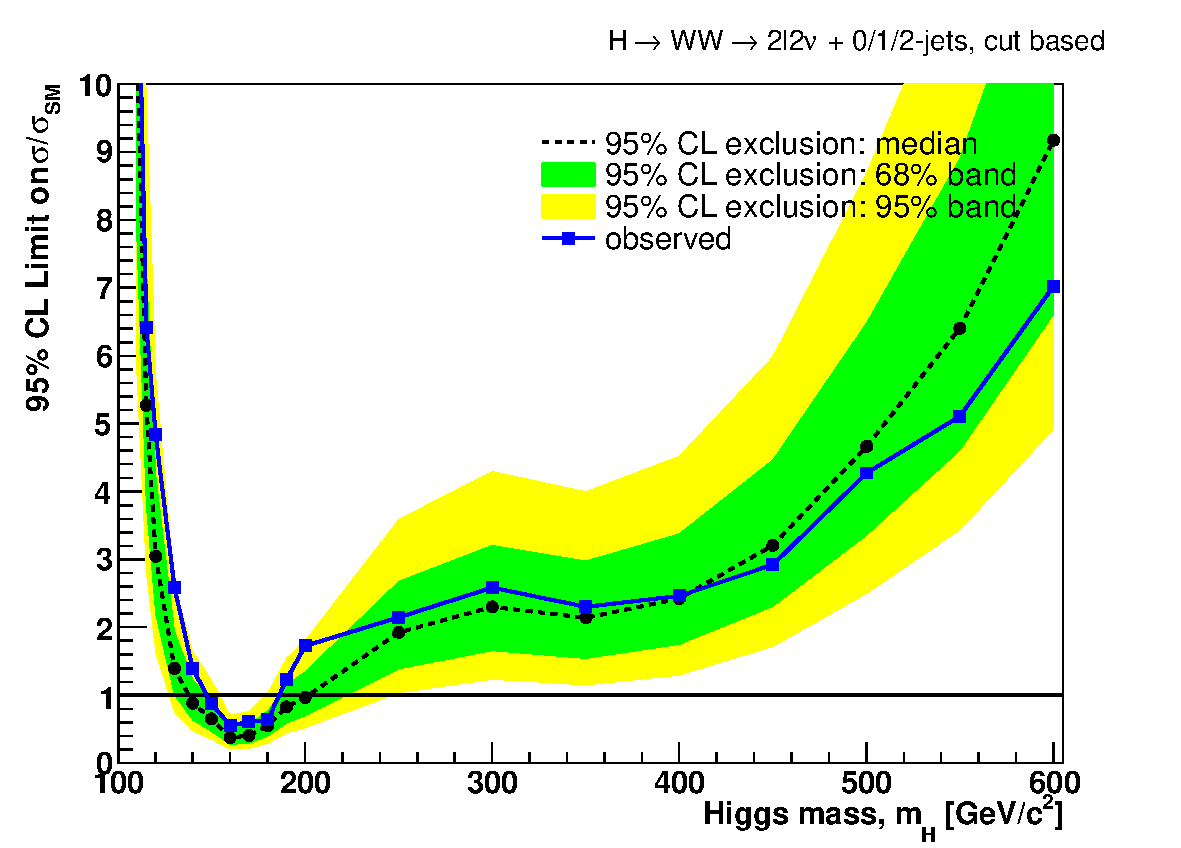
\includegraphics[width=.45\textwidth]{figures/limits_nj_cut-CLs-asymptotic_EPS.pdf}}
\subfigure[SM Higgs (shape-based)]{
\centering
\label{subfig:sm_cut_zoom}
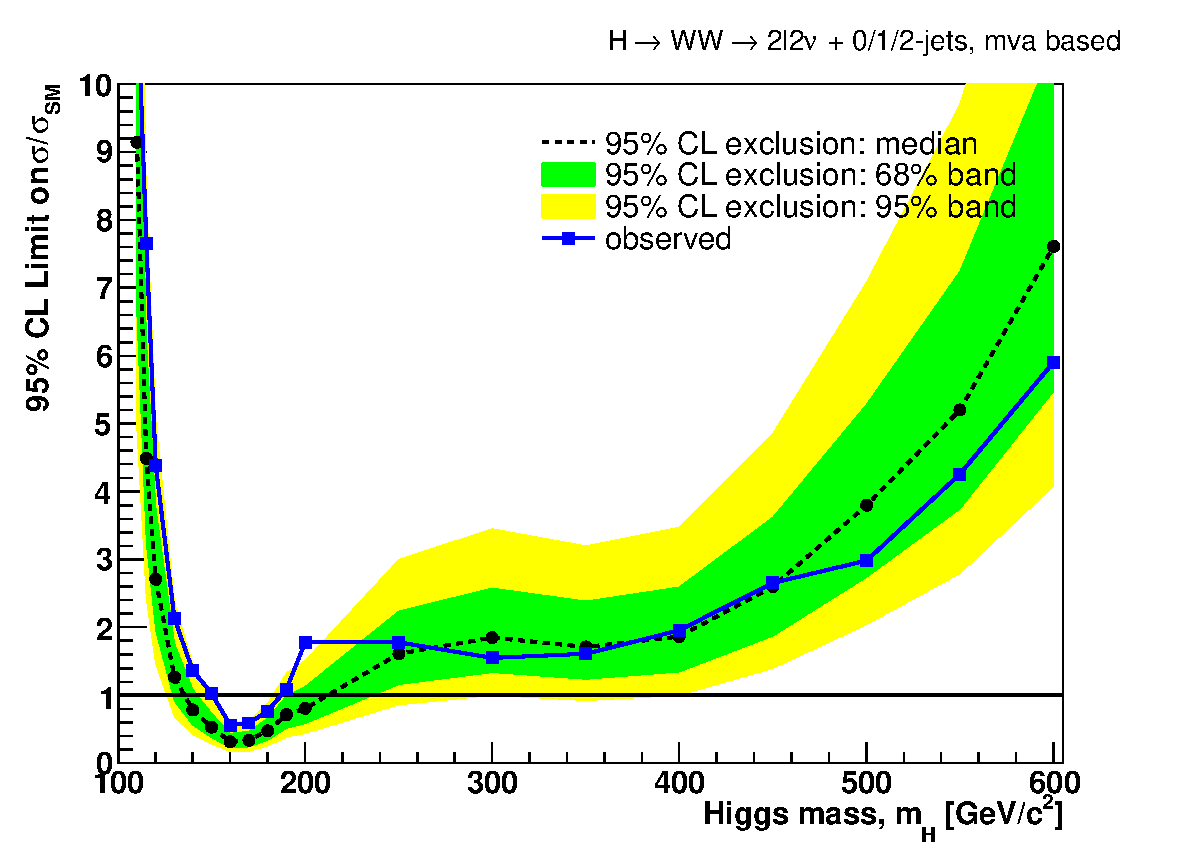
\includegraphics[width=.45\textwidth]{figures/limits_nj_shape-CLs-asymptotic_EPS.pdf}}

\caption{Expected and observed upper limits on the SM using EPS dataset.}
\label{fig:uls_eps}
\end{figure}
